\documentclass[12pt]{beamer}
\usetheme{CambridgeUS}
\usepackage[utf8]{inputenc}
\usepackage[spanish]{babel}
\usepackage{amsmath}
\usepackage{amsfonts}
\usepackage{amssymb}
\usepackage{graphicx}
\author{Kevin Garcia - Alejandro Vargas}
\title{Modelo de regresión lineal múltiple}
%\setbeamercovered{transparent} 
%\setbeamertemplate{navigation symbols}{} 
%\logo{} 
%\institute{} 
%\date{} 
%\subject{} 
\begin{document}

\begin{frame}
\titlepage
\end{frame}

%\begin{frame}
%\tableofcontents
%\end{frame}

\begin{frame}
\frametitle{Análisis exploratorio de datos}
~\\ Para trabajar con la base de datos denominada 'cadata', generamos un número aleatorio con la ayuda del software R, el cuál nos arrojó el número 15529, por tanto nuestra base de datos final, quedo con las 9 variables (columnas) y con las filas desde la 15529 hasta la 16028.

~\\ El objetivo del estudio es ajustar un modelo de regresión para la variable 'Valor medio de la casa', tomando como variables explicativas las variables 'Ingreso medio','Edad media de la vivienda', 'Total de habitaciones','Total de dormitorios','Población','Hogares','Latitud' y 'Longitud'. 
\end{frame}

\begin{frame}
\frametitle{Análisis exploratorio de datos}
~\\ Previo al ajuste e interpretación del modelo, se llevo a cabo el respectivo análisis exploratorio de datos, para tener una idea de las descriptivas mas importantes de cada variable, su forma de distribución y su rango de valores.
\end{frame}

\begin{frame}
\frametitle{Análisis exploratorio de datos}
\begin{figure}[!h]
    \begin{center}
        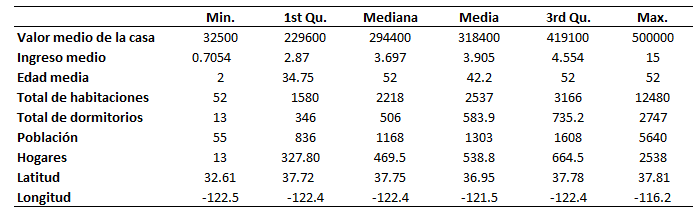
\includegraphics[width=12cm]{imagenes/estadisticas.png}
        \caption{Resumen estadístico}
        \label{fig:Densidad}
    \end{center}
\end{figure}

\end{frame}
\begin{frame}
\frametitle{Variable 'Valor mediano de las viviendas'}
\begin{figure}[!h]
    \begin{center}
        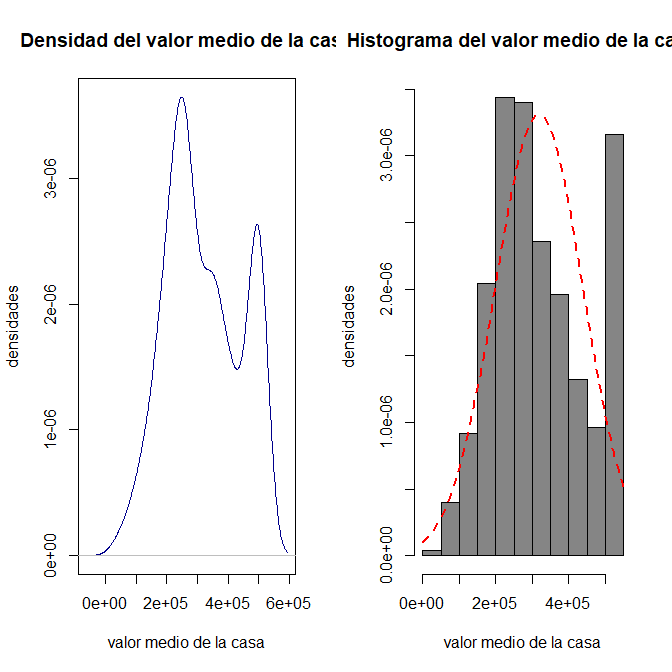
\includegraphics[width=11cm]{imagenes/1.png}
        \caption{Histograma y densidad de la variable 'Valor mediano de las casas'}
        \label{fig:Densidad}
    \end{center}
\end{figure}
\end{frame}
\begin{frame}
\frametitle{Variable 'Valor mediano de las viviendas'}
\begin{figure}[!h]
    \begin{center}
        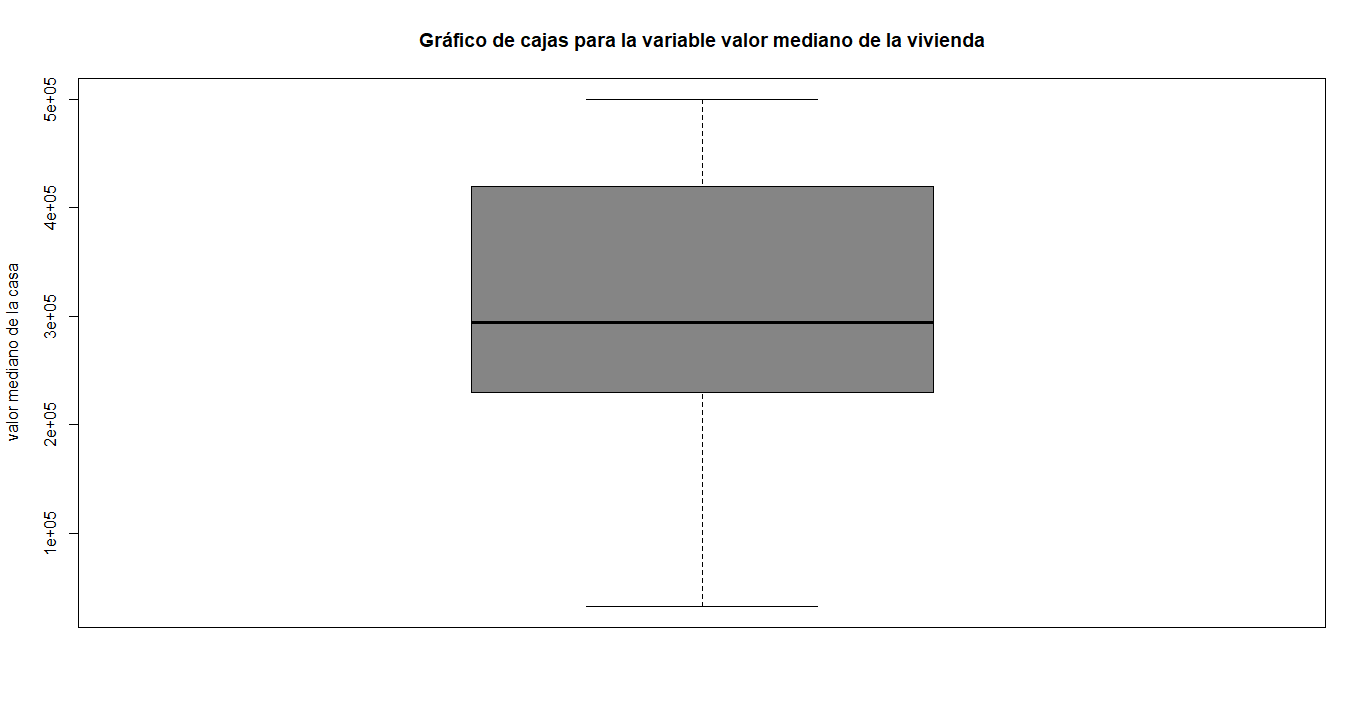
\includegraphics[width=11cm]{imagenes/12.png}
        \caption{Gráfico de cajas para la variable 'Valor mediano de las casas'}
        \label{fig:Densidad}
    \end{center}
\end{figure}
\end{frame}

\begin{frame}
\frametitle{Variable 'Ingreso mediano'}
\begin{figure}[!h]
    \begin{center}
        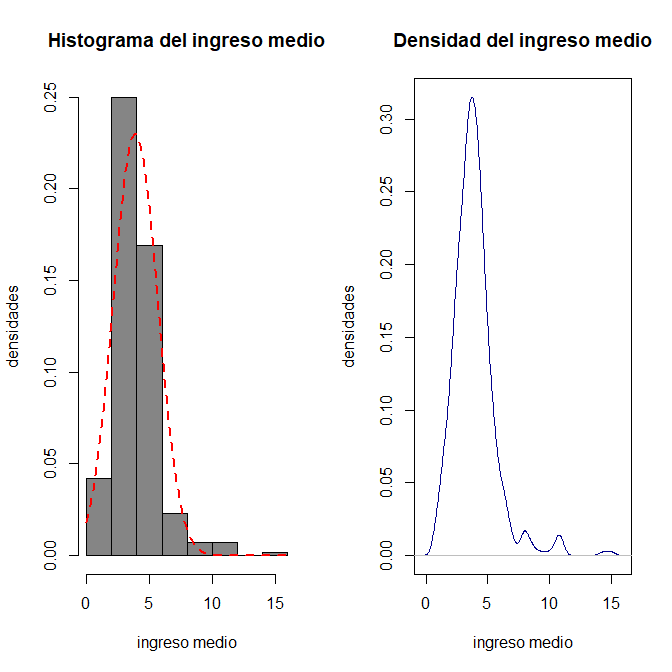
\includegraphics[width=11cm]{imagenes/2.png}
        \caption{Histograma y densidad de la variable 'Ingreso mediano'}
        \label{fig:Densidad}
    \end{center}
\end{figure}
\end{frame}
\begin{frame}
\frametitle{Variable 'Ingreso mediano'}
\begin{figure}[!h]
    \begin{center}
        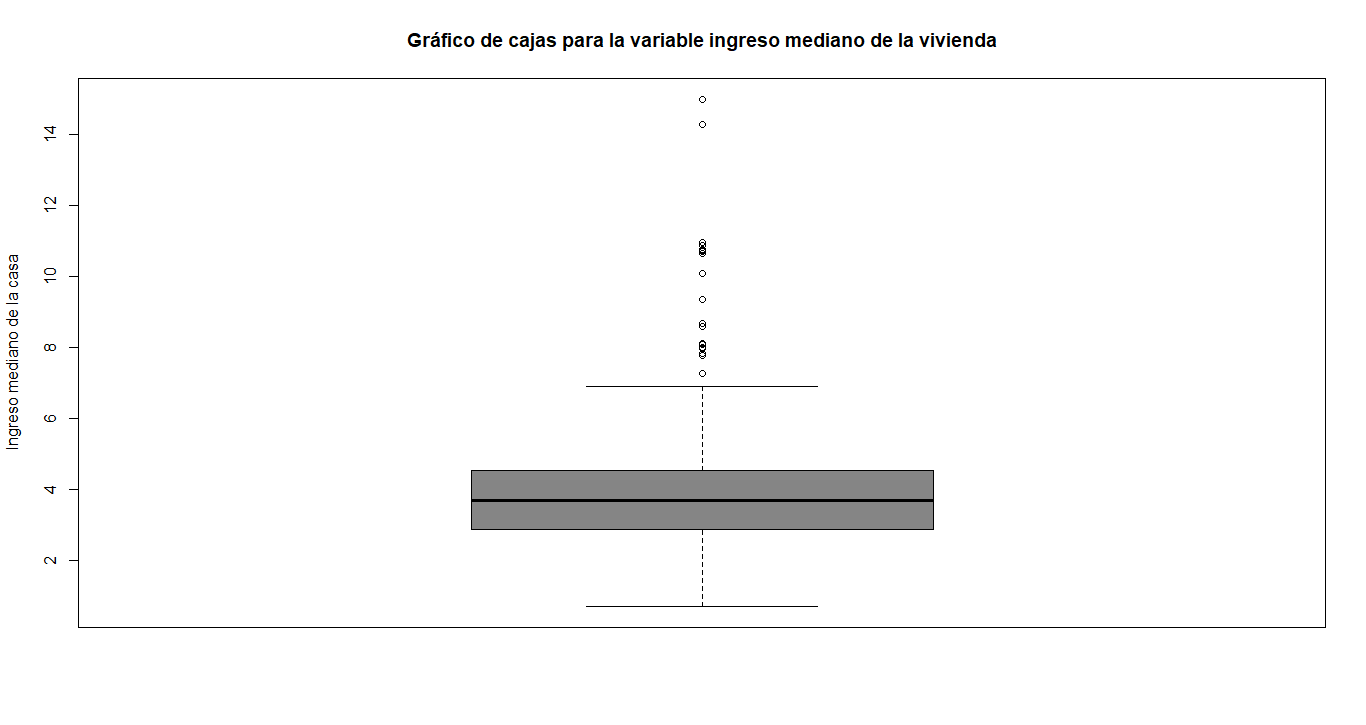
\includegraphics[width=11cm]{imagenes/13.png}
        \caption{Gráfico de cajas para la variable 'Ingreso mediano de las casas'}
        \label{fig:Densidad}
    \end{center}
\end{figure}
\end{frame}

\begin{frame}
\frametitle{Variable 'Edad mediana de las viviendas'}
\begin{figure}[!h]
    \begin{center}
        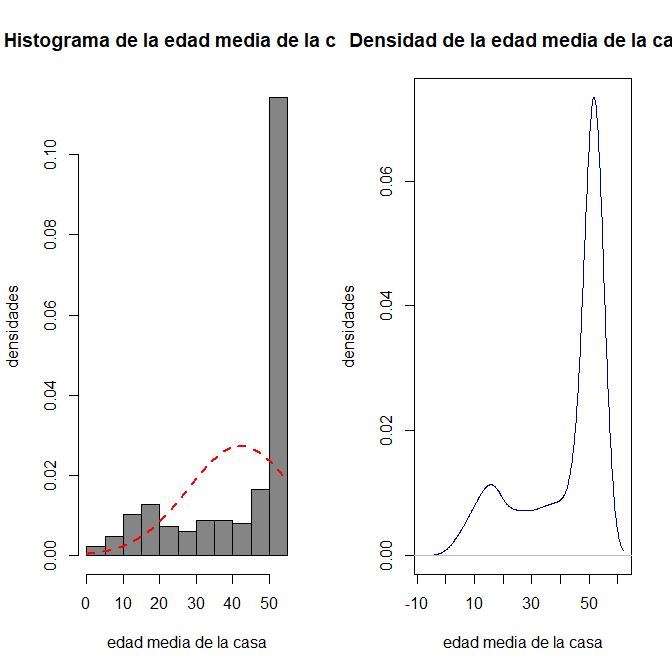
\includegraphics[width=11cm]{imagenes/3.png}
        \caption{Histograma y densidad de la variable 'Edad mediana de las viviendas'}
        \label{fig:Densidad}
    \end{center}
\end{figure}
\end{frame}
\begin{frame}
\frametitle{Variable 'Edad mediana de las viviendas'}
\begin{figure}[!h]
    \begin{center}
        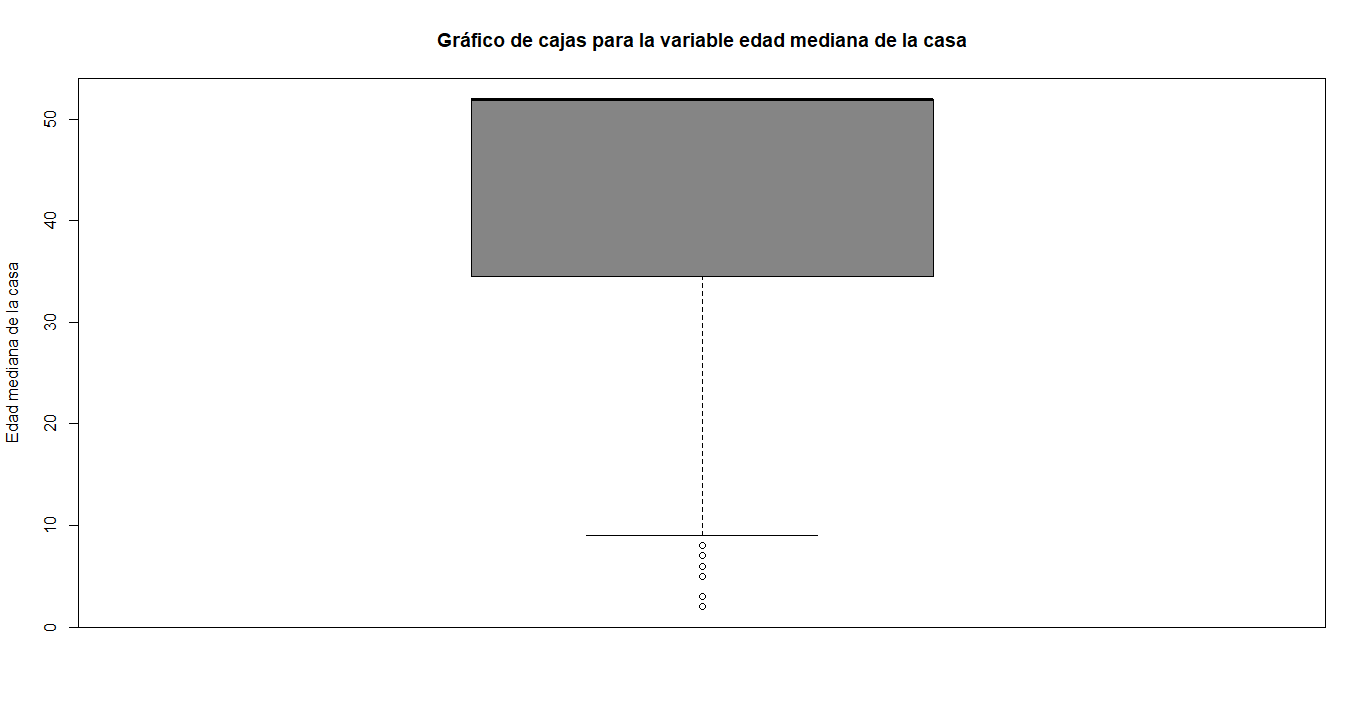
\includegraphics[width=11cm]{imagenes/14.png}
        \caption{Gráfico de cajas para la variable 'Edad mediana de las viviendas'}
        \label{fig:Densidad}
    \end{center}
\end{figure}
\end{frame}

\begin{frame}
\frametitle{Variable 'Total de habitaciones'}
\begin{figure}[!h]
    \begin{center}
        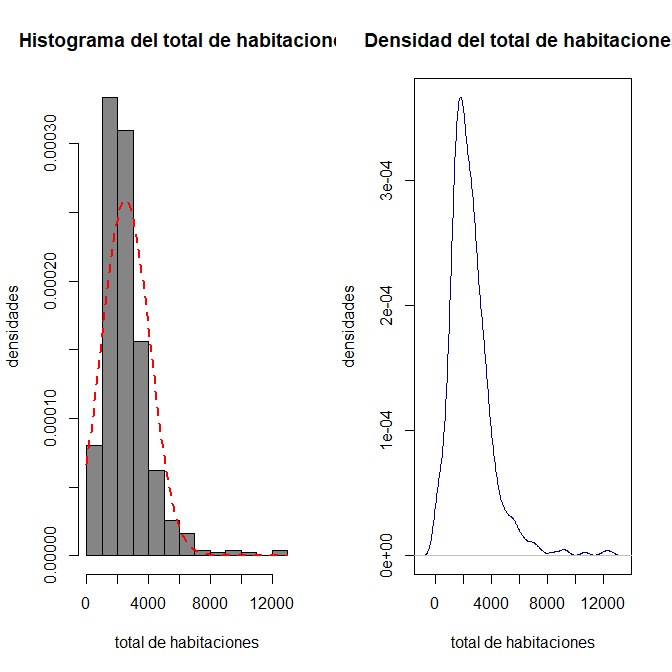
\includegraphics[width=11cm]{imagenes/4.png}
        \caption{Histograma y densidad de la variable 'Total de habitaciones'}
        \label{fig:Densidad}
    \end{center}
\end{figure}
\end{frame}
\begin{frame}
\frametitle{Variable 'Total de habitaciones'}
\begin{figure}[!h]
    \begin{center}
        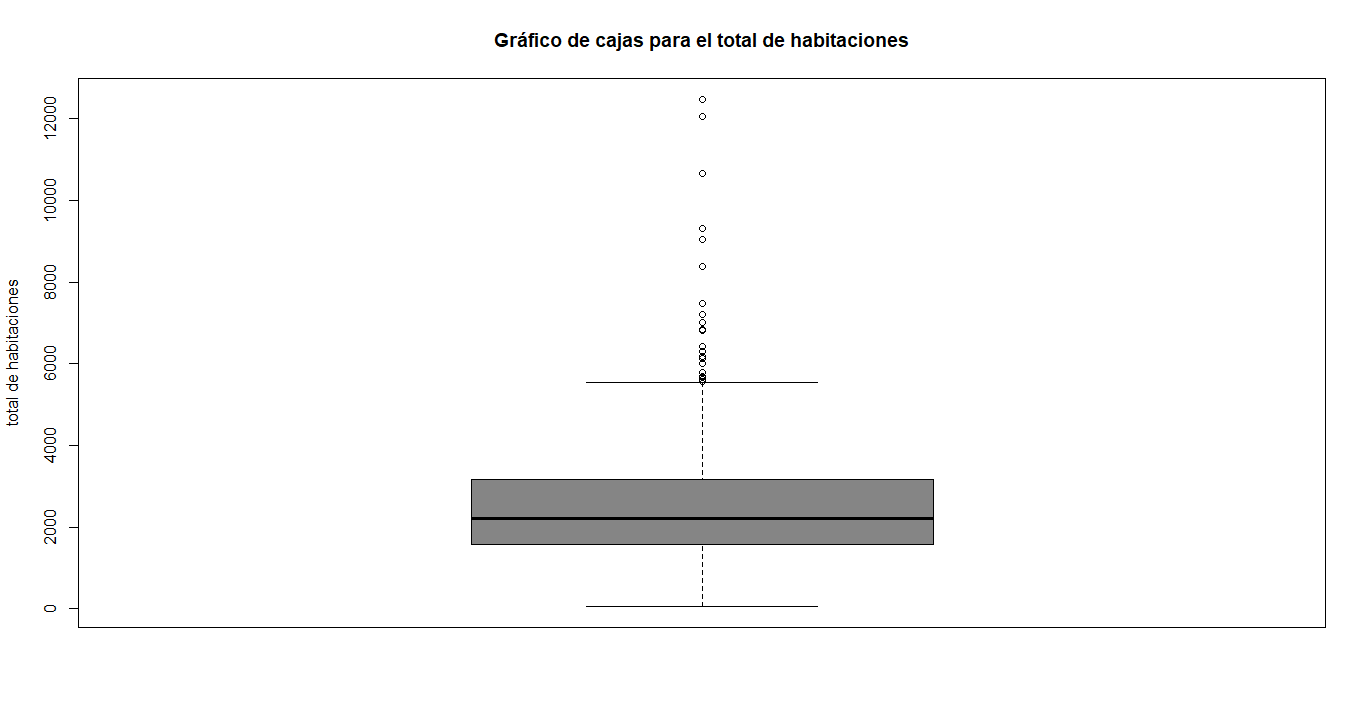
\includegraphics[width=11cm]{imagenes/15.png}
        \caption{Gráfico de cajas para la variable 'Total de habitaciones'}
        \label{fig:Densidad}
    \end{center}
\end{figure}
\end{frame}

\begin{frame}
\frametitle{Variable 'Total de dormitorios'}
\begin{figure}[!h]
    \begin{center}
        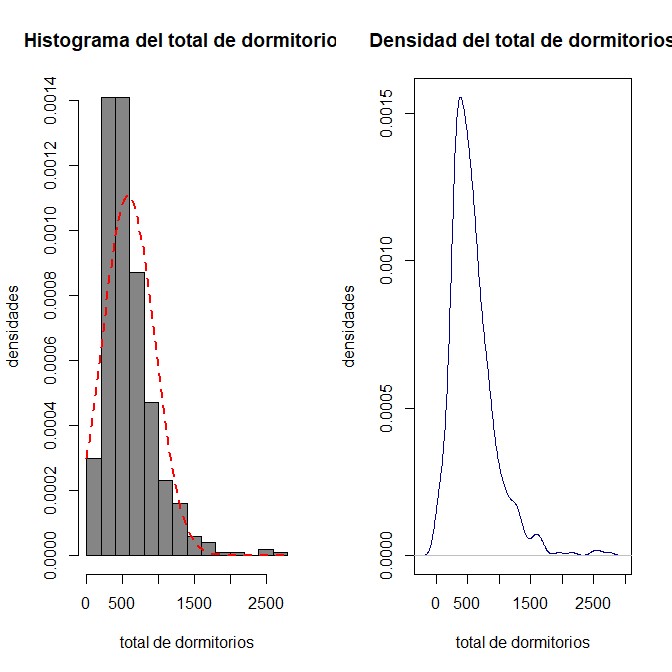
\includegraphics[width=11cm]{imagenes/5.png}
        \caption{Histograma y densidad de la variable 'Total de dormitorios'}
        \label{fig:Densidad}
    \end{center}
\end{figure}
\end{frame}
\begin{frame}
\frametitle{Variable 'Total de dormitorios'}
\begin{figure}[!h]
    \begin{center}
        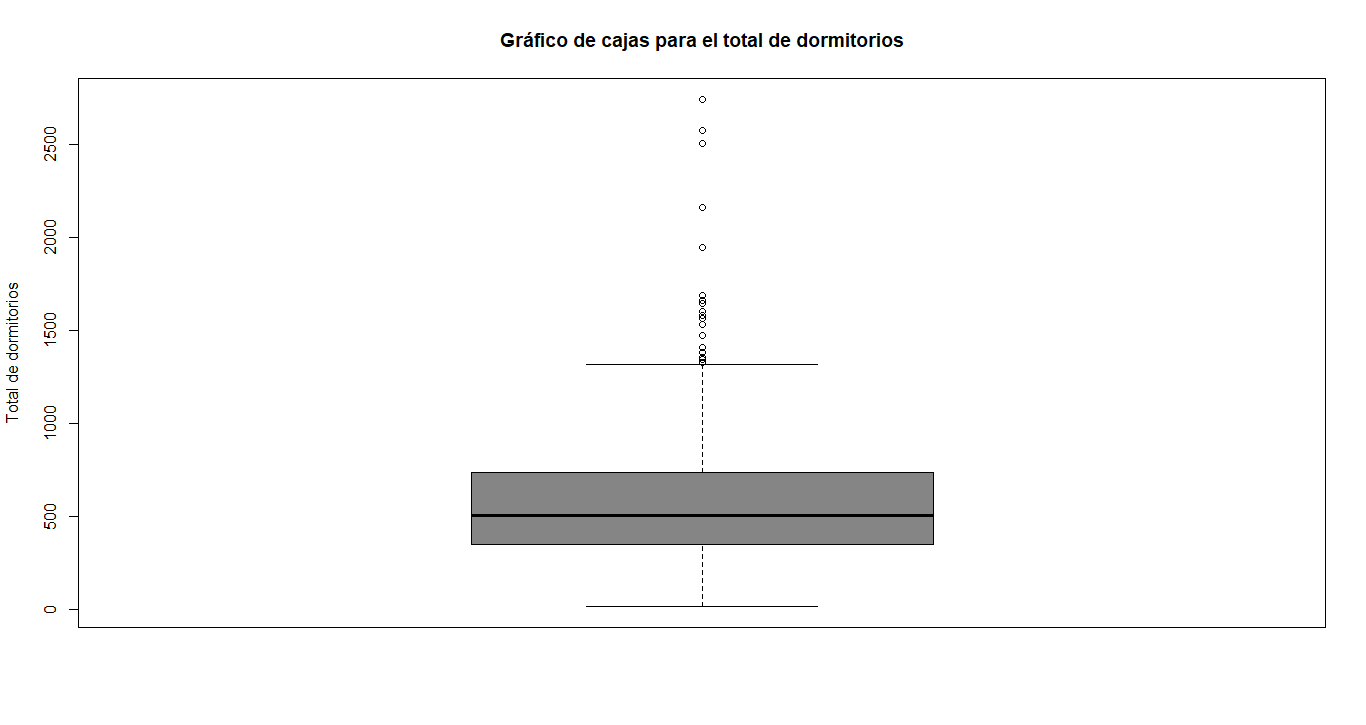
\includegraphics[width=11cm]{imagenes/16.png}
        \caption{Gráfico de cajas para la variable 'Total de dormitorios'}
        \label{fig:Densidad}
    \end{center}
\end{figure}
\end{frame}
\begin{frame}
\frametitle{Variable 'Población'}
\begin{figure}[!h]
    \begin{center}
        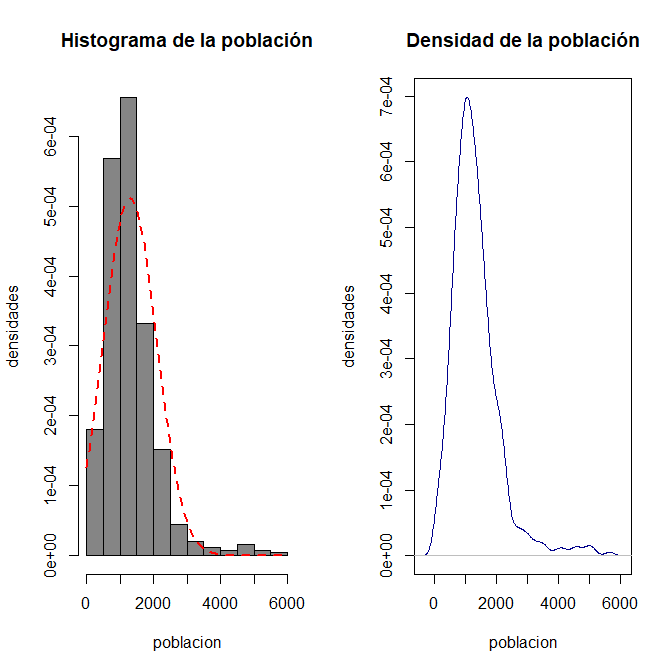
\includegraphics[width=11cm]{imagenes/6.png}
        \caption{Histograma y densidad de la variable 'Población'}
        \label{fig:Densidad}
    \end{center}
\end{figure}
\end{frame}
\begin{frame}
\frametitle{Variable 'Población'}
\begin{figure}[!h]
    \begin{center}
        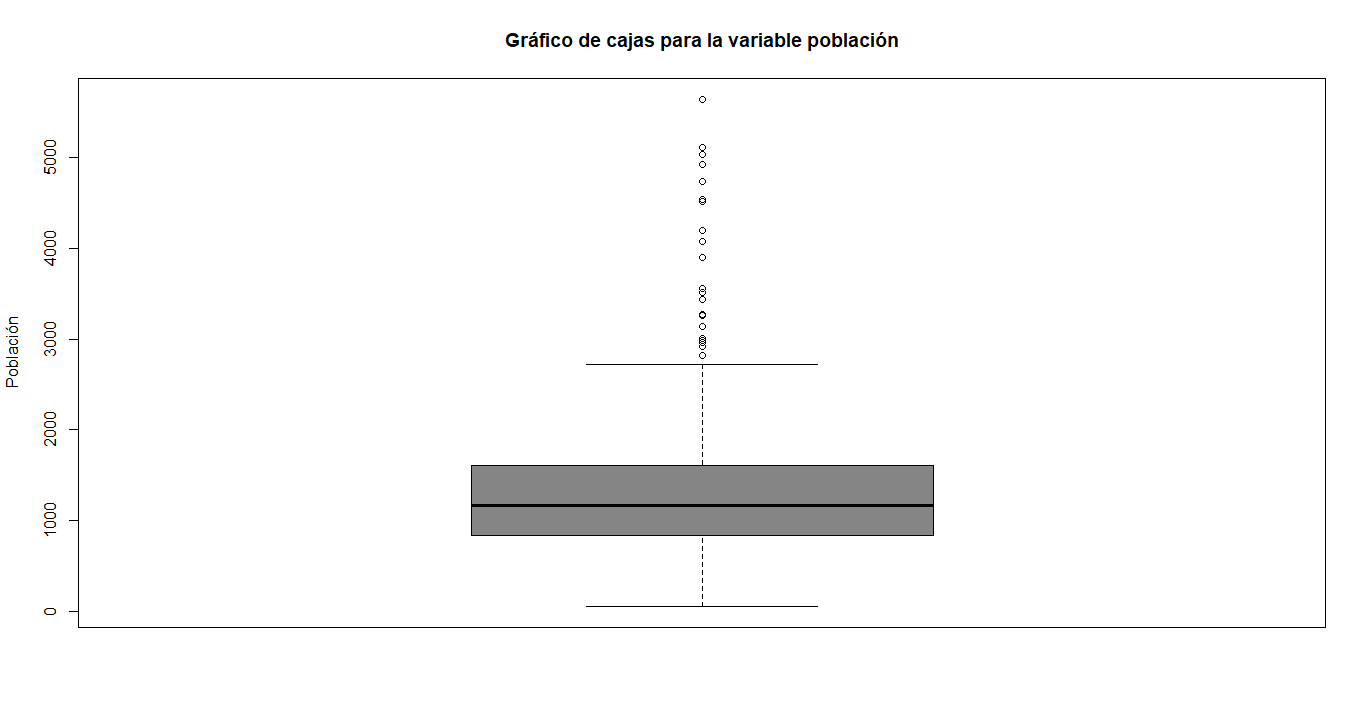
\includegraphics[width=11cm]{imagenes/17.png}
        \caption{Gráfico de cajas para la variable 'Población'}
        \label{fig:Densidad}
    \end{center}
\end{figure}
\end{frame}

\begin{frame}
\frametitle{Variable 'Hogares'}
\begin{figure}[!h]
    \begin{center}
        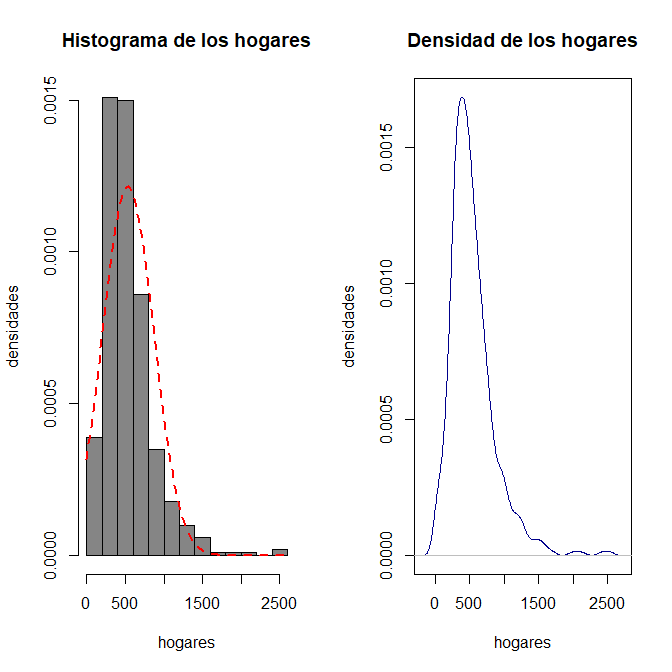
\includegraphics[width=11cm]{imagenes/7.png}
        \caption{Histograma y densidad de la variable 'Hogares'}
        \label{fig:Densidad}
    \end{center}
\end{figure}
\end{frame}
\begin{frame}
\frametitle{Variable 'Hogares'}
\begin{figure}[!h]
    \begin{center}
        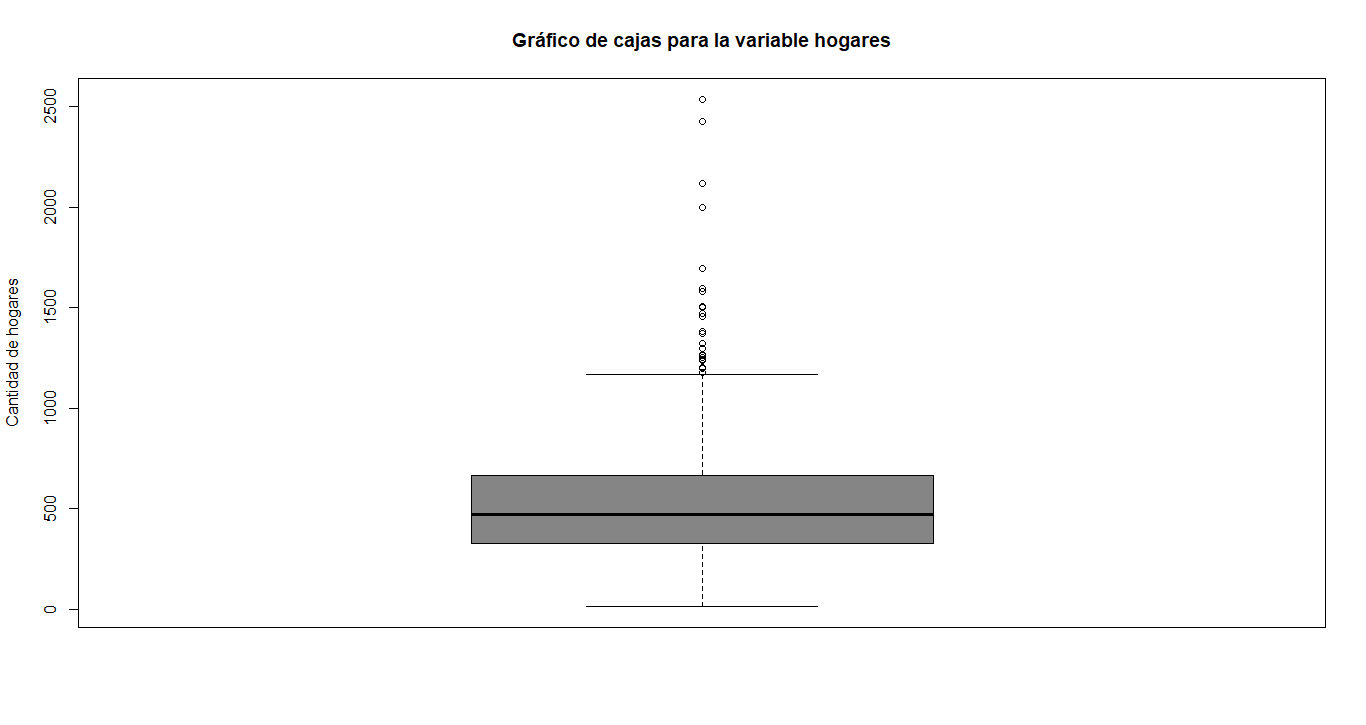
\includegraphics[width=11cm]{imagenes/18.png}
        \caption{Gráfico de cajas para la variable 'Hogares'}
        \label{fig:Densidad}
    \end{center}
\end{figure}
\end{frame}

\begin{frame}
\frametitle{San Francisco}
\begin{figure}[!h]
    \begin{center}
        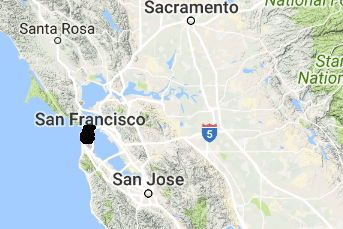
\includegraphics[width=11cm]{imagenes/sanfransisco.png}
        \caption{Mapa con los puntos dados de longitud y latitud}
        \label{fig:Densidad}
    \end{center}
\end{figure}
\end{frame}

\begin{frame}
\frametitle{San Diego}
\begin{figure}[!h]
    \begin{center}
        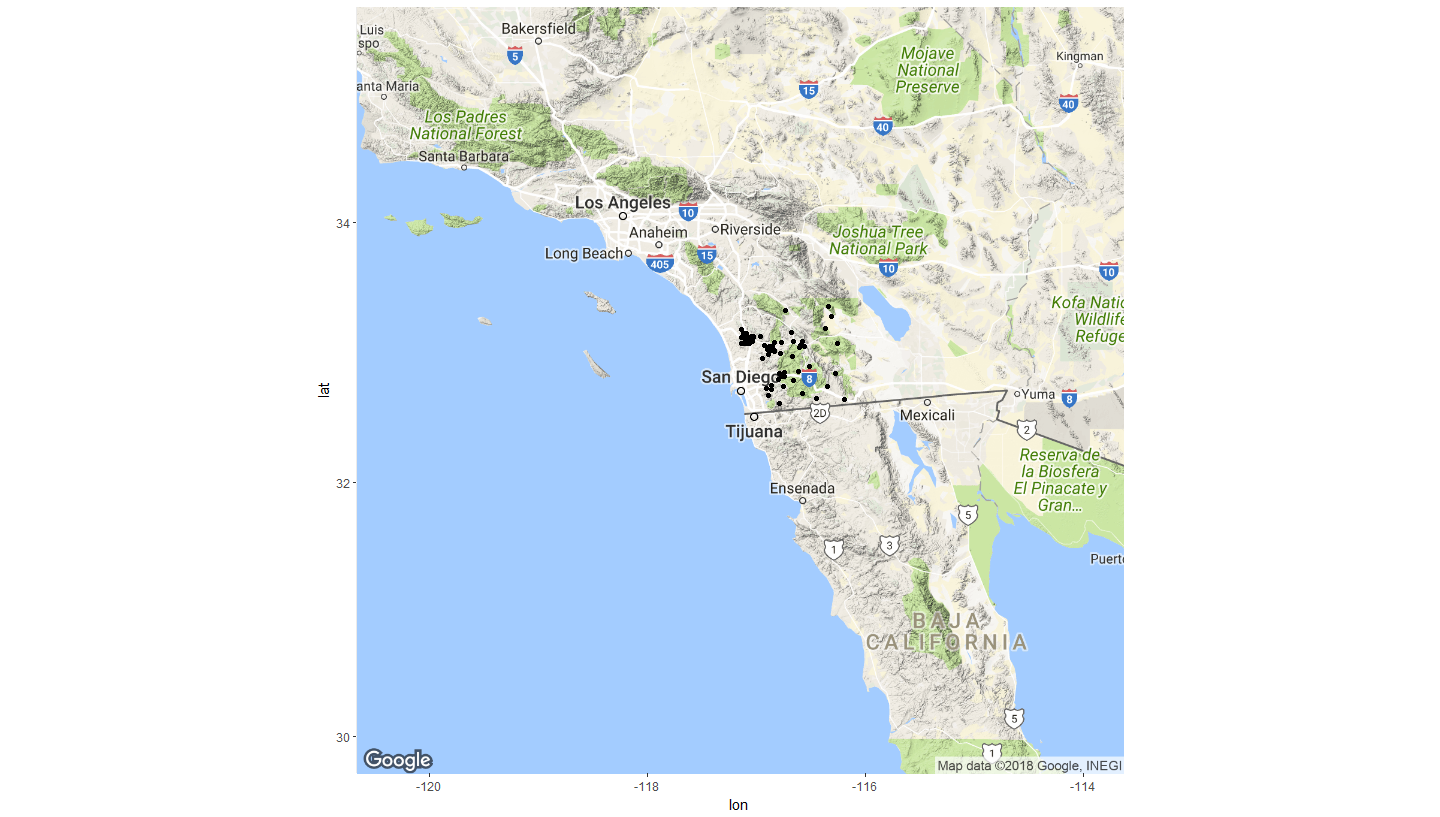
\includegraphics[width=11cm]{imagenes/sandiego.png}
        \caption{Mapa con los puntos dados de longitud y latitud}
        \label{fig:Densidad}
    \end{center}
\end{figure}
\end{frame}

\begin{frame}
\frametitle{Posibles relaciones entre las variables explicativas}
\begin{itemize}
\item Variables 'Población' y 'Hogares':
\begin{figure}[!h]
    \begin{center}
        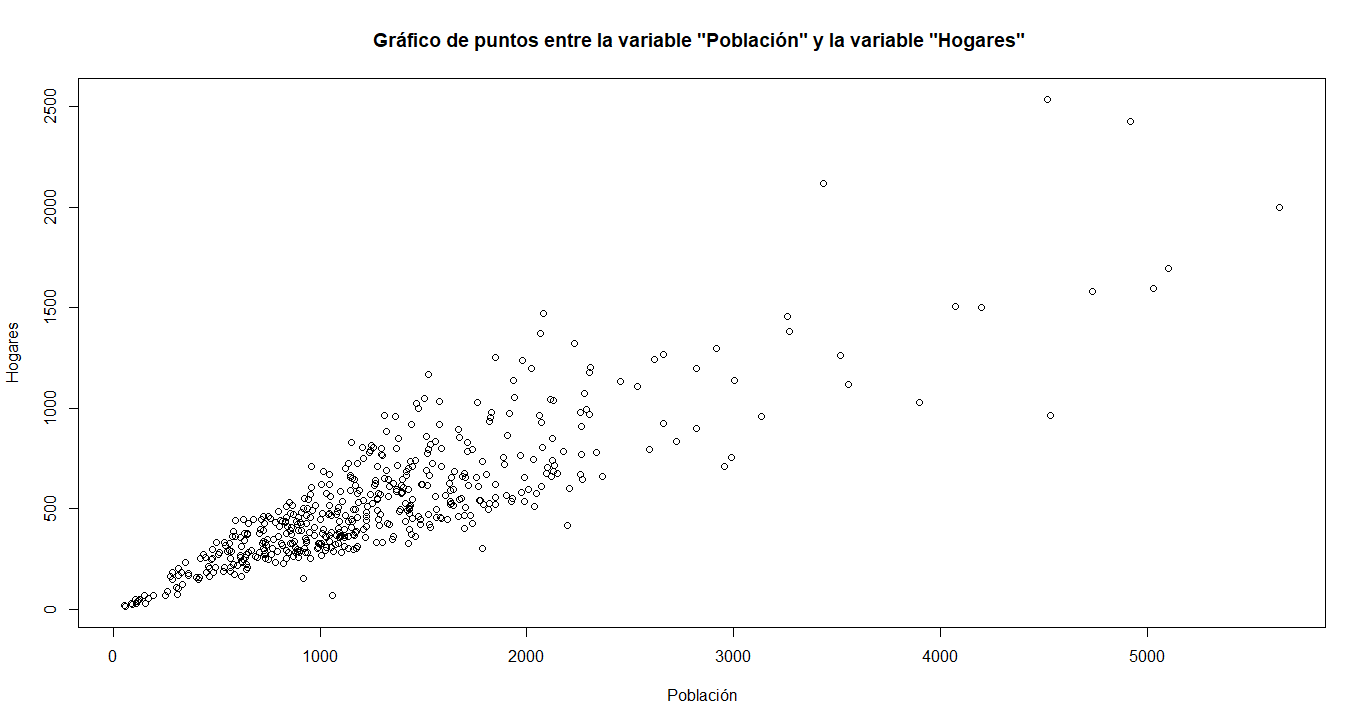
\includegraphics[width=10cm]{imagenes/10.png}
        \caption{Gráfico de puntos entre las variables 'Población' y 'Hogares'}
        \label{fig:Densidad}
    \end{center}
\end{figure}
\end{itemize}
\end{frame}

\begin{frame}
\frametitle{Posibles relaciones entre las variables explicativas}
\begin{itemize}
\item correlación de Pearson: $r=0.853918$
\item correlación de Spearman: $\rho=0.8395669$
\end{itemize}
\end{frame}

\begin{frame}
\frametitle{Posibles relaciones entre las variables explicativas}
\begin{itemize}
\item Variables 'total de habitaciones' y 'total de dormitorios':
\begin{figure}[!h]
    \begin{center}
        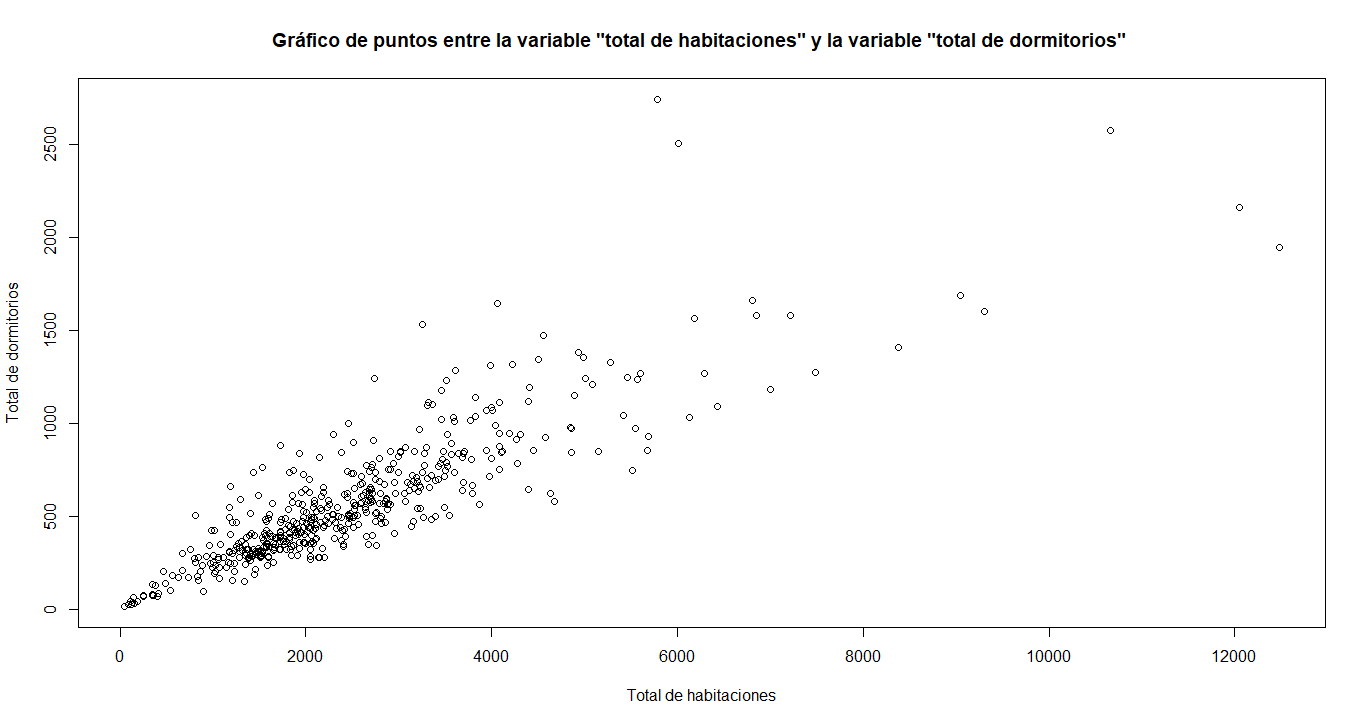
\includegraphics[width=10cm]{imagenes/11.png}
        \caption{Gráfico de puntos entre las variables 'total de habitaciones' y 'total de dormitorios'}
        \label{fig:Densidad}
    \end{center}
\end{figure}
\end{itemize}
\end{frame}

\begin{frame}
\frametitle{Posibles relaciones entre las variables explicativas}
\begin{itemize}
\item correlación de Pearson: $r=0.862072$
\item correlación de Spearman: $\rho=0.8716658$
\end{itemize}
\end{frame}

\begin{frame}
\frametitle{Modelo ajustado e interpretación}
~\\ El modelo ajustado incluyendo todas las variables sin transformación y sin selección de variables es:
~\\ $Y=-4113000+22100 X_{1}+1835 X_{2}+30.35 X_{3}-14.43 X_{4}-
124.5 X_{5}+210.2 X_{6}-
33230 X_{7}-45080 X_{8}$

~\\ Donde: Y=Valor mediano de la casa, $X_{1}=$Ingreso mediano, $X_{2}=$Edad mediana de la vivienda, $X_{3}=$Total de habitaciones, $X_{4}=$Total de dormitorios, $X_{5}=$Población, $X_{6}=$Hogares, $X_{7}=$Latitud, $X_{8}=$Longitud.
\end{frame}

\begin{frame}
\frametitle{Modelo ajustado e interpretación}
\begin{itemize}
\item $\beta_{0}$:Representa el valor del intercepto con el eje y, esto quiere decir que -4113000 siempre va a afectar mi variable dependiente sin importar en cuantas unidades aumente mis otras variables.  
\item $\beta_{1}$:por cada unidad que aumente de ingreso mediano se aumentan 22100 unidades del valor mediano de la casa.
\item $\beta_{2}$:por cada unidad que aumente de edad mediana de la vivienda se aumentan 1835 unidades del valor mediano de la casa.
\item $\beta_{3}$:por cada unidad que aumente de total de habitaciones se aumentan 30,35 unidades del valor mediano de la casa.
\item $\beta_{4}$:por cada unidad que aumente de total de dormitorios se disminuye 14,43 unidades del valor mediano de la casa.
\end{itemize}
\end{frame}
\begin{frame}
\begin{itemize}
\item $\beta_{5}$:por cada unidad que aumente de población se disminuye 124,5 unidades del valor mediano de la casa.
\item $\beta_{6}$:por cada unidad que aumente de hogares se disminuye 210,2 unidades del valor mediano de la casa.
\item $\beta_{7}$:por cada unidad que aumente de latitud se disminuye 33230 unidades del valor mediano de la casa.
\item $\beta_{8}$:por cada unidad que aumente de longitud se disminuye 45080 unidades del valor mediano de la casa.
\end{itemize}
\end{frame}
\end{document}